\documentclass{article}
%\documentclass[hyperref={colorlinks=true}]{beamer}
%\documentclass[handout,hyperref={colorlinks=true}]{beamer}


%%%%%%%%%%%%%%%%%%%%%%%%%%%%%%Paquetes%%%%%%%%%%%%%%%%%%%%%%%%%%%%%%%%%%%%%%%%%%%%%%%5
%%%%%%%%%%%%%%%%%%%%%%%%%%%%%%%%%%%%%%%%%%%%%%%%%%%%%%%%%%%%%%%%%%%%%%%%%%%%%%%%%%%%%
\usepackage{empheq}
\usepackage[spanish]{babel}
\usepackage[utf8x]{inputenc}
\usepackage{times}
%\usepackage[T1]{fontenc}
\usepackage{amssymb,amsmath}
\usepackage{enumerate}
\usepackage{verbatim}
\usepackage{ esint }
%\usepackage{pst-all}
%\usepackage{pstricks-add}
\usepackage{array}
%\usepackage[T1]{fontenc}
\usepackage{animate}
%\usepackage{media9}
\usepackage{xparse}
\usepackage{listings}
\usepackage{ wasysym }
%\usepackage{sagetex}
\usepackage{yfonts,mathrsfs,eufrak}
\usepackage{hyperref}
\usepackage{color}
\usepackage{url}
\usepackage{theorem}
\usepackage{boiboites}
\usepackage{wrapfig}
\usepackage{ esint }
\definecolor{mygreen}{rgb}{0,0.6,0}
\definecolor{mygray}{rgb}{0.5,0.5,0.5}
\definecolor{mymauve}{rgb}{0.58,0,0.82}

\lstset{ %
  backgroundcolor=\color{white},   % choose the background color; you must add \usepackage{color} or \usepackage{xcolor}
  basicstyle=\footnotesize,        % the size of the fonts that are used for the code
  breakatwhitespace=false,         % sets if automatic breaks should only happen at whitespace
  breaklines=true,                 % sets automatic line breaking
  captionpos=b,                    % sets the caption-position to bottom
  commentstyle=\color{mygreen},    % comment style
  deletekeywords={...},            % if you want to delete keywords from the given language
  escapeinside={\%*}{*)},          % if you want to add LaTeX within your code
  extendedchars=true,              % lets you use non-ASCII characters; for 8-bits encodings only, does not work with UTF-8
  frame=single,	                   % adds a frame around the code
  keepspaces=true,                 % keeps spaces in text, useful for keeping indentation of code (possibly needs columns=flexible)
  keywordstyle=\color{blue},       % keyword style
  language=Python,                 % the language of the code
  otherkeywords={*,...},           % if you want to add more keywords to the set
  numbers=left,                    % where to put the line-numbers; possible values are (none, left, right)
  numbersep=5pt,                   % how far the line-numbers are from the code
  numberstyle=\tiny\color{mygray}, % the style that is used for the line-numbers
  rulecolor=\color{black},         % if not set, the frame-color may be changed on line-breaks within not-black text (e.g. comments (green here))
  showspaces=false,                % show spaces everywhere adding particular underscores; it overrides 'showstringspaces'
  showstringspaces=false,          % underline spaces within strings only
  showtabs=false,                  % show tabs within strings adding particular underscores
  stepnumber=2,                    % the step between two line-numbers. If it's 1, each line will be numbered
  stringstyle=\color{mymauve},     % string literal style
  tabsize=2,	                   % sets default tabsize to 2 spaces
  title=\lstname                   % show the filename of files included with \lstinputlisting; also try caption instead of title
}


%%%%%%%%%%%%%%%%%%%%%%%%%%Nuevos comandos entornos%%%%%%%%%%%%%%%%%%%%%%%%%%%%%%%%
%%%%%%%%%%%%%%%%%%%%%%%%%%%%%%%%%%%%%%%%%%%%%%%%%%%%%%%%%%%%%%%%%%%%%%%%
\newenvironment{demo}{\noindent\emph{Dem.}}{$\square$ \newline\vspace{5pt}}

\newcommand{\com}{\mathbb{C}}
\newcommand{\dis}{\mathbb{D}}
\newcommand{\rr}{\mathbb{R}}
\newcommand{\oo}{\mathcal{O}}
\renewcommand{\emph}[1]{\textcolor[rgb]{1,0,0}{#1}}
\newcommand{\der}[2]{\frac{\partial #1}{\partial #2}}
\renewcommand{\v}[1]{\overrightarrow{#1}}
\renewcommand{\epsilon}{\varepsilon}
%\newcommand{\defverbatim}{\def{#1}}
\renewenvironment{frame}[1]{}{}
\newcommand{\qed}{$\square$}
\DeclareMathOperator{\atan2}{atan2}
\DeclareMathOperator{\sen}{sen}


%%%%%%%%%%%%%%%%%%%%%%%%Colores
\definecolor{myblue}{rgb}{.8, .8, 1}
\definecolor{dblackcolor}{rgb}{0.0,0.0,0.0}
\definecolor{dbluecolor}{rgb}{0.01,0.02,0.7}
\definecolor{dgreencolor}{rgb}{0.2,0.4,0.0}
\definecolor{dgraycolor}{rgb}{0.30,0.3,0.30}
\newcommand{\dblue}{\color{dbluecolor}\bf}
\newcommand{\dred}{\color{dredcolor}\bf}
\newcommand{\dblack}{\color{dblackcolor}\bf}


%%%%%%%%%%Definimos una caja con color
\newlength\mytemplen
\newsavebox\mytempbox
\makeatletter
\newcommand\mybluebox{%
\@ifnextchar[%]
{\@mybluebox}%
{\@mybluebox[0pt]}}
\def\@mybluebox[#1]{%
\@ifnextchar[%]
{\@@mybluebox[#1]}%
{\@@mybluebox[#1][0pt]}}
\def\@@mybluebox[#1][#2]#3{
\sbox\mytempbox{#3}%
\mytemplen\ht\mytempbox
\advance\mytemplen #1\relax
\ht\mytempbox\mytemplen
\mytemplen\dp\mytempbox
\advance\mytemplen #2\relax
\dp\mytempbox\mytemplen
\colorbox{myblue}{\hspace{1em}\usebox{\mytempbox}\hspace{1em}}}
\makeatother
\DeclareDocumentCommand\boxedeq{ m g }{%
{\begin{empheq}[box={\mybluebox[2pt][2pt]}]{equation}% #1%
\IfNoValueF {#2} {\label{#2}}%
#1
\end{empheq}
}%
}


%%%%%%%%%%%%%%%%%%
\newboxedtheorem[boxcolor=orange, background=blue!5, titlebackground=blue!20,
titleboxcolor = black,thcounter=section]{problema}{Problema}{thcounter1}

\newboxedtheorem[boxcolor=orange, background=blue!5, titlebackground=blue!20,
titleboxcolor = black,thcounter=section]{teorema}{Teorema}{thcounter2}

\newboxedtheorem[boxcolor=orange, background=blue!5, titlebackground=blue!20,
titleboxcolor = black,thcounter=section]{definicion}{Definici\'on}{thcounter3}

\newboxedtheorem[boxcolor=orange, background=blue!5, titlebackground=blue!20,
titleboxcolor = black,thcounter=section]{lema}{Lema}{thcounter4}

\newboxedtheorem[boxcolor=orange, background=blue!5, titlebackground=blue!20,
titleboxcolor = black,thcounter=section]{corolario}{Corolario}{thcounter5}

\newboxedtheorem[boxcolor=orange, background=blue!5, titlebackground=blue!20,
titleboxcolor = black,thcounter=section]{proposicion}{Proposici\'on}{thcounter6}

\newboxedtheorem[boxcolor=orange, background=blue!5, titlebackground=blue!20,
titleboxcolor = black,thcounter=section]{codigo}{Función SymPy}{}




\newcounter{ejemplo_cont}
\setcounter{ejemplo_cont}{1}

\newenvironment{ejemplo}{\noindent\textbf{Ejemplo  \arabic{ejemplo_cont}.} }{\addtocounter{ejemplo_cont}{1}}
%%%%%%%%%%%%%%%%%%%%%%%%%%%%%%%%%%%%%%%%%%%%%%%%%%%%%%%%%%%%%%%%%%%%%%%%%%%%%%%%%%%%%%%%%%%%%%%%%%%%%%%%%%%
%%%%%%%%%%Para escibir en clase articulo o similar






\title{Teoría de Lie y ecuaciones diferenciales}


%%%%%%%%%%%%%%%%%%%%%%%%%%%%%%%%%%%%%%%%%%%%%%%%%%%%%%%%%%%%%%%%%%%%%%%%%%%%%%%%%%%%%%


\begin{document}

  \maketitle
  \begin{center}
   
\includegraphics[scale=0.2]{imagenes/unrc.jpg}
   \end{center}

\tableofcontents



\section{Introducción histórica}





<<Marius Sophus Lie fue un matemático noruego (17 de diciembre de 1842-18 de febrero de 1899) que creó en gran parte la teoría de la simetría continua, y la aplicó al estudio de la geometría y las ecuaciones diferenciales.
La herramienta principal de Lie, y uno de sus logros más grandes fue el descubrimiento de que los grupos continuos de transformación (ahora llamados grupos de Lie), podían ser
 entendidos mejor "linealizándolos", y estudiando los correspondientes campos vectoriales generadores (los, así llamados, generadores infinitesimales).
Los generadores obedecen una versión linealizada de la ley del grupo llamada el corchete o conmutador, y tienen la estructura de lo que hoy, en honor suyo, llamamos un álgebra de Lie.>> (Wikipedia)
 \marginpar{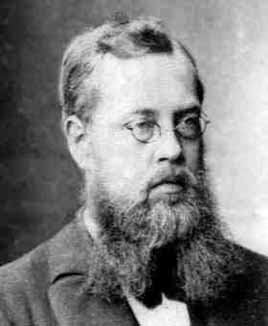
\includegraphics[scale=.28]{imagenes/Sophus_Lie.jpg}
}





\section{Formas Diferenciales, una introducción ingenua}

Como ya se mencionó, ecuación ecuación diferencial general de primer orden:

\boxedeq{\frac{dy}{dx}=f(x,y)}{eq:gral_orden1}
puede ser escrita como \emph{forma diferencial}
\boxedeq{M(x,y)dx+N(x,y)dy=0}{eq:gral_orden1_FormDif}

 La primera expresión es más asimétrica, entre las variables $x$ e $y$ una de ellas es independiente ($x$) y la otra independiente  ($y$).  La segunda expresión es  más simétrica, las dos variables tienen el mismo estatus.

 Las expresiones del tipo \eqref{eq:gral_orden1_FormDif} representan un ente matemático importante llamado \href{http://es.wikipedia.org/wiki/Forma_diferencial}{forma diferencial}. No disponemos del tiempo necesario para dotar con entidad matemática el concepto de forma diferencial. Tampoco  resulta de vital importancia. Pero las reglas que rigen la combinación de las formas diferenciales son muy simples y nos gustaría describir este aspecto de las formas diferenciales brevemente; como motivación para un estudio posterior más profundo y para que el lector gane en confianza en su manipulación. Daremos así una pintura de las formas diferenciales incompleta, por cuanto sólo diremos como ellas se combinan pero no contestaremos la pregunta de que son. Sólo digamos, para advertir al lector sobre los requisítos teóricos que se requieren, que las formas diferenciales se encuentran asociados al concepto de variedad diferencial, concepto este que generaliza al de curva y superficie.  Más 
concretamente, las formas diferenciales son funciones que toman valores en los duales de los espacios tangentes a las variedades diferenciales. En particular hay formas diferenciales asociadas a los espacios euclideo, que podemos identificar con  $\rr^n$.

Aqui vamos a pensar a las formas diferenciales como objetos puramente formales sobre los que actúa un operador $d$, leyes de composición internas y externas. Se construyen formas diferenciales invocando un sistema de coordenadas $x_1,\ldots,x_n$. Estas coordenadas, deben ser coordenadas de alguna variedad diferencial, pero, por simplicidad, supondremos que son coordenadas cartesianas ortogonales de un espacio euclideo. Las formas diferenciales forman un espacio vectorial con una operación de suma $+$ y producto por un escalar. Además tienen definido un producto $\wedge$, llamado \href{https://es.wikipedia.org/wiki/Producto_exterior}{producto exterior}, que posee  algunas particularidades.  Como los polinomios, las formas diferenciales tienen grado. Por eso se dice que forman un álgebra graduada. A diferencia de los polinomios, este grado no supera la dimensión $n$ del espacio ($\rr^n$ o más generalmente una variedad) a la que están asociadas. Para ser más exactas, la única forma de 
grado $k>n$ es la trivial, esto es la nula. Denotamos $\Lambda_k$ las formas de grado $k$, siendo $\Lambda =\bigoplus_{k=0}^{n}\Lambda_k$ el espacio vectorial de todas ellas. Luego $d:\Lambda\to\Lambda$ y $\wedge:\Lambda\times\Lambda\to \Lambda$. Ahora describimos unas simples reglas de las formas,  $d$ y $\wedge$.



\begin{enumerate}
   \item Una 0-forma diferencial es una función $g(x_1,\ldots,x_n)$.

  \item Si $\alpha\in\Lambda_k$ y $\beta\in\Lambda_p$ entonces $\alpha \wedge \beta\in \Lambda_{k+p}$.
  \item El producto $\wedge$ es asociativo, distributivo y satisface una especia de anticonmutatividad, especídficamente si $\alpha\in\Lambda_k$ y $\beta\in\Lambda_p$ entonces $\alpha\wedge \beta=(-1)^{kp}\beta\wedge\alpha$. En particular $\alpha\wedge\alpha=0$ cuando $\alpha$ es un $k$-forma con $k$ impar.
  \item El diferencial satisface
  \begin{enumerate}
    \item Si $\omega$ es una $k$-forma diferencial $d\omega$ es una $k+1$ forma diferencial.
    \item  $d^2\omega=d(d\omega)=0$, para toda $\omega\in\Lambda$.
    \item Si $\alpha\in\Lambda_k$ entonces  $d(\alpha\wedge\beta)=d\alpha\wedge\beta+(-1)^k\alpha\wedge d\beta$.
    \item En el caso de $0$-forma (función) $g(x_1,\ldots,x_n)$ el diferencial se define
    \[dg=\frac{\partial g}{\partial x_1}dx_1+\cdots+\frac{\partial g}{\partial x_n}dx_n\]

  \end{enumerate}
  \item Las expresiones $dx_i$, $i=1,\ldots,n$ forman una especie de base del espacio de las formas $\Lambda$, en el sentido que cualquier $k$ forma $\alpha$ se expresa de la siguiente manera:
  \[\alpha=\sum_{1\leq i_1<\cdots i_k\leq n}g_{i_1\ldots i_k} dx_{i_1}\wedge\cdots\wedge dx_{i_n},\]
  para ciertas funciones $g_{i_1\ldots i_k}$. Observar que la suma se extiende sobre todos los subconjuntos ordenados de $\{1,\ldots,n\}$.
\end{enumerate}


Una $k$-forma diferencial $\alpha$ se llama \href{https://es.wikipedia.org/wiki/Formas_diferenciales_cerradas_y_exactas}{exacta} cuando es el diferencial de una $k-1$-forma y se dice \href{https://es.wikipedia.org/wiki/Formas_diferenciales_cerradas_y_exactas}{cerrada} cuando $d\alpha=0$. Las propiedades de las formas implican que toda forma exacta es cerrda. Un famoso \href{https://es.wikipedia.org/wiki/Formas_diferenciales_cerradas_y_exactas#Lema_de_Poincar.C3.A9}{Lema de Poincare} trata con el recíproco de esta afirmación.

Las reglas anteriores permiten computar cualquiera de las operaciones.
\begin{ejemplo} Si $\alpha=M(x,y)dx+N(x,y)dy$ es una 1-forma de $\rr^2$, entonces
\[ \begin{split}
    d\alpha&=dM\wedge dx-Md^2x + dN\wedge dy-Nd^2y\\
    &=\left(\frac{\partial M}{\partial x}dx+ \frac{\partial M}{\partial y}dy\right)\wedge dx+
    \left(\frac{\partial N}{\partial x}dx+ \frac{\partial N}{\partial y}dy\right)\wedge dy\\
    &= \left(\frac{\partial N}{\partial x}- \frac{\partial M}{\partial y}\right) dx\wedge dy
   \end{split}
\]
Recordemos el famoso \href{https://es.wikipedia.org/wiki/Teorema_de_Green}{Teorema de Green}, que afirmaba que si $D\subset \rr^2$ era una región cuyo borde $C=\partial D$ era una curva cerrada simple, entonces
\[\ointctrclockwise_{\partial D} Mdx +Ndy=\iint_D \left(\frac{\partial N}{\partial x}- \frac{\partial M}{\partial y}\right) dx dy.\]
Utilizando formas diferenciales este resultado se escribe de la manera, mucho más compacta y sugerente
\[\ointctrclockwise_{\partial D} \alpha = \iint_Dd\alpha,\]
donde $\alpha =M(x,y)dx+N(x,y)dy$.  Esto es una relación clave de las formas diferenciales que se generaliza en un teorema fundamental de la matemática llamado \href{https://es.wikipedia.org/wiki/Teorema_de_Stokes}{Teorema de Stokes}.
\end{ejemplo}




\begin{ejemplo} Computemos $d^2g$, cuando $g$ es una función (0-forma).

\[
\begin{split}
d^2g&=d\left(\frac{\partial g}{\partial x_1}dx_1+\cdots+\frac{\partial g}{\partial x_n}dx_n\right)\\
&= d\left(\frac{\partial g}{\partial x_1}\right)\wedge dx_1+\cdots+d\left(\frac{\partial g}{\partial x_n}\right)\wedge dx_n
    -\frac{\partial g}{\partial x_1}\wedge d^2x_1-\cdots-\frac{\partial g}{\partial x_n}\wedge d^2x_n\\
    &=\left(\sum_{i=1}^n\frac{\partial^2g}{\partial x_i\partial x_1} dx_i\right)\wedge dx_1+\cdots+\left(\sum_{i=1}^n\frac{\partial^2g}{\partial x_i\partial x_n} dx_i\right)\wedge dx_n\\
    &= \sum_{i\neq 1}^n\frac{\partial^2g}{\partial x_i\partial x_1} dx_i\wedge dx_1+\cdots
    \sum_{i\neq n}^n\frac{\partial^2g}{\partial x_i\partial x_n} dx_i\wedge dx_n\\
    &=\sum_{1\leq i<j\leq n}^n\left\{\frac{\partial^2g}{\partial x_i\partial x_j}- \frac{\partial^2g}{\partial x_j\partial x_i}\right \} dx_i\wedge dx_j=0.
\end{split}
\]
Que es lo que tenía que ser.


\end{ejemplo}




\section{Cambios de Variables}

\begin{problema}[Cambio de variables]
 Dada la ecuación \eqref{eq:gral_orden1} o \eqref{eq:gral_orden1_FormDif} en las variables $x,y$. Queremos encontrar nuevas variables $\hat{x}=\hat{x}(x,y)$ y $\hat{y}=\hat{y}(x,y)$ tales que la ecuación se transforme en una que podamos resolver.
\end{problema}






\subsection{Cómputos de cambiamos variables}
Vamos a estudiar en primer lugar como computar cambios de variables, item que suele ofrecer cierta resistencia al estudiante, a pesar de que es sencillo. Empezaremos por casos más sencillos hasta ir a la situación más general.

\subsubsection{Cambio de la variable dependiente manteniendo la independiente}

Supongamos que el conjunto de variables se relacionan  por la identidad $y=y(x,\hat{y})$. Nos conviene en este caso partir de la relación inversa. Entoces por la regla de la cadena (que sería más apropiado llamarla regla de cambio de variables para la derivada)

\[\frac{dy}{dx}=\frac{\partial h}{\partial x}+\frac{\partial h}{\partial \hat{y}}\frac{d\hat{y}}{dx}.\]

La ecuación se convierte

\[\frac{\partial y}{\partial x}+\frac{\partial y}{\partial \hat{y}}\frac{d\hat{y}}{dx}=f(x,y(x,\hat{y})).\]
Que es una expresión sólo en $\hat{y}$ y $x$. Parece más complicada, pero en un ejemplo concreto puede ser más simple.







\begin{ejemplo} Hacer el cambio de variable en la  ecuación indicados
\[y=\frac{e^{\hat{y}}}{x}\quad\text{en}\quad  y'=\left[\ln(xy)\right]^2xy-\frac{y}{x}.\]
 1) Expresemos $dy/dx$ sólo con $x$, $\hat{y}$ y $d\hat{y}/dx$.
\[\frac{dy}{dx}=-\frac{e^{\hat{y}}}{x^2}+\frac{e^{\hat{y}}}{x}\frac{d\hat{y}}{dx}.\]
 2) Remplacemos $y'$ e $y$ en la ecuación
\[-\frac{e^{\hat{y}}}{x^2}+\frac{e^{\hat{y}}}{x}\frac{d\hat{y}}{dx}=\left[\ln\left(x \frac{e^{\hat{y}}}{x} \right)\right]^2x\frac{e^{\hat{y}}}{x}-\frac{\frac{e^{\hat{y}}}{x} }{x}.\]
 3) Simplifiquemos
\boxedeq{\frac{d\hat{y}}{dx}=\hat{y}^2x.}{}




\end{ejemplo}

Lo podemos hacer con \texttt{SymPy}, lo cual es muy útil por dos motivos. El primero porque nos permite hacer cambios de variables en expresiones muy grandes, resolviendo operaciones que a mano son sumamente tediosas. El segundo, y no menos importante para nosotros, es que es muy rico explorar un procedimiento enmarcándolo en un contexto muy distinto. En este caso, el procedimiento es relizar un cambio de variables y estamos explorando el mismo a través de un breve código que lo implementa en un lenguaje de programación.

\begin{lstlisting}
from sympy import *
x=symbols('x') #unico simbolo primitivo
y_n=Function('y_n')(x) #declaro las varaibles nuevas, funciones de las viejas
y=exp(y_n)/x #relacion entre y, y_n
eq=Eq(y.diff(x)-(ln(x*y))**2*x*y+y/x,0) #la ecuacion
simplify(eq) # simplifica expresiones
\end{lstlisting}
Obtenemos la ecuación
\[\frac{1}{x} \left(- x \log^{2}{\left (e^{\operatorname{y\_n}{\left (x \right )
}} \right )} + \frac{d}{d x} \operatorname{y\_n}{\left (x \right )}\right) e^{
\operatorname{y\_n}{\left (x \right )}} = 0\]
que \texttt{SymPy} no simplifica a nuestro gusto




\subsubsection{Cambio de la variable independiente manteniendo la dependiente}

Supongamos  $\hat{x}=\hat{x}(x)$. Usamos la relación
\[\frac{dy}{dx}=\frac{dy}{d\hat{x}}\frac{d\hat{x}}{dx}.\]
Suponiendo que la relación $\hat{x}=\hat{x}(x)$ se invierte en $x=x(\hat{x})$, todo lo que resta es sustituir  $x$ por su igual en términos de $\hat{x}$

\[\frac{dy}{d\hat{x}}=f(x(\hat{x}),y) \left[\left.\frac{d\hat{x}}{dx}\right|_{x=x(\hat{x})}\right]^{-1}.\]
Que es una expresión sólo en $\hat{x}$ e $y$. Describir el procedimiento  en general puede hacer parecer que es más dificil de lo que en realidad es en un caso concreto.



\begin{ejemplo} Hacer el cambio de variable en la  ecuación indicados
\[x=\cos \hat{x}\quad\text{en}\quad  -\frac{dy}{dx}+\frac{x}{\sqrt{1-x^2}}y=0.\]
1) $\hat{x}=\arcsen x$
\[\frac{dy}{dx}=\frac{dy}{d\hat{x}} \frac{d\hat{x}}{dx}  =-\frac{1}{\sqrt{1-x^2}}\frac{dy}{d\hat{x}}.\]
 2) Remplacemos $x$ e $y'$ en la ecuación
\[\frac{1}{\sqrt{1-x^2}}\frac{dy}{d\hat{x}}+ \frac{x}{\sqrt{1-x^2}}y=0\]
3) Reemplazando $x$ por $\cos(\hat{x})$ y simplificando
\[\frac{dy}{d\hat{x}}+\cos(\hat{x}) y=0.\]

\end{ejemplo}


Para hacer esto con \texttt{SymPy} (de ahora en más omitiremos la sentencia de importanción del módulo, esta operación se hace sólo una vez por sesion).


\begin{lstlisting}
from sympy import *
x,x_n=symbols('x,x_n')
x_n=acos(x)
y=Function('y')(x_n)
Ecuacion=-y.diff()+1/(sqrt(1-x**2))*y
xn=symbols('xn')
Ecuacion.subs(x,cos(xn))
\end{lstlisting}
Obtenemos la ecuación
\[\frac{y{\left (\operatorname{acos}{\left (\cos{\left (xn \right )} \right )} \right )} \cos{\left (xn \right )}}{\sqrt{- \cos^{2}{\left (xn \right )} + 1}}
+ \frac{1}{\sqrt{- \cos^{2}{\left (xn \right )} + 1}} \left. \frac{d}{d \xi_{1
}} y{\left (\xi_{1} \right )} \right|_{\substack{ \xi_{1}=\operatorname{acos}{
\left (\cos{\left (xn \right )} \right )} }}\]
Nuevamente \texttt{SymPy} no simplifica a nuestro gusto, aún aquellas expresiones que parece muy evidente como se simplifican . El lector debe tener en cuenta que en ningún momento uno le dijo a \texttt{SymPy} que tipo de ente estaba manipulando en expresiones del tipo \texttt{x\_n=acos(x)}. Le pudo parecer natural que eran números reales, puesto es eso lo que matemáticamente son para nosotros, no obstante esta información nunca fue comunicada al interprete de \texttt{SymPy}. ¿Porqué el habría de entender que \texttt{x} es real? Si al fin y al cabo \texttt{x\_n=acos(x)} tiene sentido si \texttt{x} es complejo y aún si es una matríz. Muchas veces las operaciones que se simplifican en un campo no lo pueden hacer en otro. El comando  \texttt{symbols} tiene la opción de informar a \texttt{SymPy} que tipo de ente representa \texttt{x} de la siguiente forma
\texttt{x=symbols('x',real=True)}. Usandoló de esta forma se consiguen mejores resultados en las simplificaciones.


\subsection{Cambio de variable general $\hat{x}=\hat{x}(x,y)$, $\hat{y}=\hat{y}(x,y)$}
\begin{enumerate}
  \item Calculamos $d\hat{y}/d\hat{x}$ en las variables $x,y$
    \boxedeq{
      \frac{d\hat{y}}{d\hat{x}}=\frac{\frac{d\hat{y}}{dx}}{\frac{d\hat{x}}{dx}}=\frac{\frac{\partial\hat{y}}{\partial x}+\frac{\partial\hat{y}}{\partial y}y'}{\frac{\partial\hat{x}}{\partial x}+\frac{\partial\hat{x}}{\partial y}y'}=\frac{\frac{\partial\hat{y}}{\partial x}+\frac{\partial\hat{y}}{\partial y}f(x,y)}{\frac{\partial\hat{x}}{\partial x}+\frac{\partial\hat{x}}{\partial y}f(x,y)}.
	    }{eq:subsder}

   \item En la expresión resultante sustituímos $x,y$ por las tansformaciones 			inversas $x=x(\hat{x},\hat{y})$ y  $y=y(\hat{x},\hat{y})$
\end{enumerate}



\begin{ejemplo} Transformar a polares:
  \[\frac{dy}{dx}=\frac{y^3+x^2y-x-y}{x^3+xy^2-x+y}.\]
\end{ejemplo}

\begin{ejemplo} Transformar a polares
 \[
  \frac{dy}{dx}=\frac{y^3+x^2y-x-y}{x^3+xy^2-x+y}.
 \]
\end{ejemplo}
 
Dado que el cálculo es extenso lo haremos con \texttt{SymPy}, el procedimiento seguido ilustra como hacerlo a mano. Es ilustrativo hacer esto último para apreciar la utilidad de usar un sistema de álgebra computacional (SAC) como \texttt{SymPy}.



\begin{lstlisting}
from sympy import *
x=symbols('x')
y=Function('y')(x)
r=sqrt(x**2+y**2)
theta=atan(y/x)
Expr2=r.diff(x)/theta.diff(x)
\end{lstlisting}

Obtenemos la siguiente expresión 
\[\frac{dr}{d\theta}=\frac{\frac{dr}{dx}}{\frac{d\theta}{dx}}=\frac{\left(1 + \frac{1}{x^{2}} y^{2}{\left (x \right )}\right) \left(x + y{\left (x \right )} \frac{d}{d x} y{\left (x \right )}\right)}{\sqrt{x^{2} + y^{2}{\left (x \right )}} \left(\frac{1}{x} \frac{d}{d x} y{\left (x \right )} - \frac{1}{x^{2}} y{\left (x \right )}\right)}.\]
Ahora sustituímos $y'(x)$ usando la ecuación diferencial, redefinimos $r,\theta$ fundamentalmente para limpiar el valor que tenían asignado en el código previo, que era una expresión de $x,y$, y finalmente sustituímos $x$e $y$ por su expresión en polares. 

\begin{lstlisting}
Expr3=Expr2.subs(y.diff(x),(y**3+x**2*y-x-y)/(x**3+x*y**2-x+y))
r,theta=symbols('r,theta',positive=True)
Expr4=Expr3.subs([(y,r*sin(theta)),(x,r*cos(theta))])
Expr5=simplify(Expr4)
\end{lstlisting}
 Encontramos que en polares la ecuación es mucho más simple
\[\frac{dr}{d\theta}=-r^3+r.\]

 Quizás  usar la notación como  forma diferencial sea más efectivo. Como $r$ y $\theta$ son funciones de $x$ e $y$, ellas son 0-formas. Usando las reglas de la diferencial, hay que reemplazar
\[
\begin{array}{ll}
x=r\cos\theta; &dx=\cos\theta dr-\sen\theta r d\theta\\
 y= r\sen\theta; & dy=\sen\theta dr+\cos\theta r d\theta\\
\end{array}
\]

 en la 1-forma:
\[(y^3+x^2y-x-y)dx-(x^3+xy^2-x+y)dy\]



 Encontramos a  \texttt{SAGE} más cómodo para operar con formas diferenciales que \texttt{SymPy}
\begin{lstlisting}
sage: r,theta=var('r,theta')
sage: U = CoordinatePatch((r,theta)) #declara coordenadas
sage: F = DifferentialForms(U) #Delara conjunto formas
sage: x= DifferentialForm(F, 0, r*cos(theta)) #define una 0-forma
sage: y= DifferentialForm(F, 0, r*sin(theta)) #define una 0-forma
sage: w=(x^3+x*y^2-x+y)*y.diff()-(y^3+x^2*y-x-y)*x.diff()#define una 1-forma
sage: w[0].simplify_full() #coeficiente de  dr
sage: w[1].simplify_full() #coeficiente de  d\theta
\end{lstlisting}
La forma obtenida es $rdr+(r^4-r^2)d\theta$.


\section{Grupos}


\subsection{Definición y ejemplos}
\begin{definicion}[Grupo]
Sean $G$ un conjunto y $\alpha$ una función tal que   $\alpha:G\times G\to G$. En el contexto de grupos es más usual la notación  $\alpha(g_1,g_2)=g_1g_2$. El par $(G,\alpha)$ se llama un grupo si se satisface
\begin{enumerate}
\item $(g_1g_2)g_3=g_1(g_2g_3)$, para todos $g_1,g_2,g_3\in G$,
\item Existe $e\in G$ tal que $eg=ge=g$,  para todo $g\in G$.
\item Para todo $g\in G$ existe $h\in G$ tal que $gh=hg=e$. Se acostumbra denotar $h=g^{-1}$.
\end{enumerate}
\end{definicion}




\begin{ejemplo} Sea $\Pi$ un plano euclideano y $G$ el conjunto de todas las transformaciones rígidas de $\Pi$ en si mismo. Entonces $G$ es un grupo con la operación de composición. Se llama el \emph{grupo de transformaciones rígidas}.
 \end{ejemplo}


\begin{ejemplo}  Sea $X=\{x_1,\ldots,x_n\}$ un conjunto de $n$ elementos y $S_n$ definido por
\[S_n=\{\sigma|\sigma:X\to X\hbox{ y }\sigma \hbox{ es biyectiva }\}\]
Entonces $S_n$ es un grupo  con la operación de composición. Se denomina \href{http://es.wikipedia.org/wiki/Grupo_simétrico}{\emph{grupo simétrico}}.
 \end{ejemplo}

\begin{ejemplo} Sea $\Delta$ un polígono regular de $n$ lados  en un plano euclideano $\Pi$ y $D_{2n}$ el conjunto de todas las transformaciones rígidas de $\Pi$ en si mismo que llevan $\Delta$ en si mismo. $D_{2n}$ se llama el \href{http://es.wikipedia.org/wiki/Grupo_diedral}{\emph{grupo diedral}}  de orden $2n$. Para un triángulo equilatero:
\begin{center}
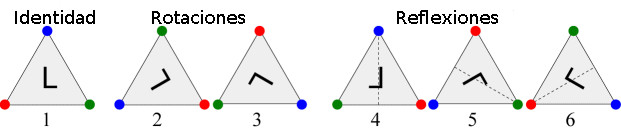
\includegraphics[scale=.4]{imagenes/SimTria.jpg}
\end{center}
\end{ejemplo}



\subsection{Teoría de grupos computacional: SAGE y GAP}

\href{http://www.gap-system.org/}{GAP - Groups, Algorithms, Programming} Lenguaje de programación para algebra discreta

\href{http://www.sagemath.org/}{SAGE:}  <<Es un sistema de software de matemáticas libre de código abierto bajo la licencia GPL. Se basa en  muchos paquetes de código abierto existentes: NumPy, SciPy, matplotlib, SymPy, Maxima, GAP, FLINT, R y muchos más. Acceda a su poder combinado a través de un lenguaje común, basado en Python. Misión: Creación de una alternativa libre de código abierto viable a Magma, Maple, Mathematica y Matlab.>>


\begin{ejemplo} Grupos con Sage.
 
\end{ejemplo}

\begin{lstlisting}
sage: G=SymmetricGroup(5)
sage: sigma=G([(1,2,3),(4,5)])
sage: sigma^2
sage: sigma^3
sage: sigma^6
sage: G.order()
sage: H=G.subgroup([sigma])
sage: H.order()
sage: H.list()
sage: H.is_normal()
sage: G1=DihedralGroup(3)
sage: G1[-2]
sage: H1=G1.subgroup(G1[-2])
sage: H1.is_normal()
sage: G1.quotient(H1)
\end{lstlisting}



\section{Grupos continuos de simetrías}

\subsection{Grupos y cambios de variables}

Los cambios de variables de un conjunto de dos variables, digamos $x$ e $y$, son funciones $\Gamma$, invertibles,  de clase $C^1$, donde $\Gamma:\Omega_1\to\Omega_2$, con $\Omega_1,\Omega_2$ abiertos de $\rr^2$.  Acostumbraremos escribir $(\hat{x},\hat{y})=\Gamma(x,y)$ y diremos que $(\hat{x},\hat{y})$ son la variables nuevas e $(x,y)$ las viejas.

 Llamaremos $\mathscr{T}$ al conjunto de todas los cambios de variables $\Gamma$.
El conjunto  $\mathscr{T}$ tiene una estructura de grupo con la operación de composición.

 El grupo de las transformaciones rígidas, los grupos diedrales $D_{2n}$, el grupo de todas las rotaciones alrededor del orígen son subgrupos de  $\mathscr{T}$.




 \begin{ejemplo} \textbf{Coordenadas polares.} Es más facil describir la transformación que lleva coordenadas polares en cartesinas. En este caso $(x,y)=\Gamma(r,\theta)$ y
\[
\begin{array}{ll}
\Gamma(r,\theta)&=(r\cos(\theta),r\sen(\theta)),\\
\Omega_1&=(0,\infty)\times (-\pi,\pi),\\
\Omega_2&=\rr^2-\{(x,y)|y=0,x\leq 0\}\\
\end{array}
\]

 \end{ejemplo}

\subsection{Grupos de Lie uniparamétricos}

\begin{definicion}[Grupos de Lie uniparamétricos]
Sea $\mathscr{T}$ el grupo de cambios de variables de $\rr^2$. Supongamos dado un homomorfismo de grupos $\Gamma:(\rr,+)\to (\mathscr{T},\circ)$.  Para $\epsilon\in\rr$ escribiremos $\Gamma_{\epsilon}=\Gamma(\epsilon)$.  Si $\Gamma_{\epsilon}(x,y)$ es diferenciable, con inversa diferenciable, respecto a $(x,y)$ y analítica respecto a $\epsilon$ diremos que $\{\Gamma_{\epsilon}|\epsilon\in\rr\}$ es un \href{http://es.wikipedia.org/wiki/Grupo_uniparamétrico}{\emph{grupo de Lie uniparamétrico de simetrías}}.
\end{definicion}


 Si $(x,y)\in\rr^2$ escribimos
  \boxedeq{(\hat{x},\hat{y})=\Gamma_{\epsilon}(x,y).}{eq:not_sim}
 Notar que $\hat{x}$, $\hat{y}$ son funciones de $x,y$ y $\epsilon$.



\begin{boite}[boxcolor=orange, background=blue!5, titlebackground=blue!20,
  titleboxcolor = black]{Propiedades de grupos de Lie uniparamétricos}
\begin{enumerate}
\item$\Gamma_{\epsilon}:\Omega_1\to\Omega_2$ es un difeomorfismo, con $\Omega_i$, $i=1,2$, abiertos de $\rr^2$.
 \item $\Gamma_{\epsilon_1}\circ \Gamma_{\epsilon_2}=\Gamma_{\epsilon_1+\epsilon_2}$.

\item $\Gamma_0=I$.

\item $\left(\Gamma_{\epsilon}\right)^{-1}=\Gamma_{-\epsilon}$

\item Las funciones  $\hat{x}(x,y,\epsilon)$ y $\hat{y}(x,y,\epsilon)$  se desarrollan en serie de potencias respecto a $\epsilon$. Es decir para todo $\epsilon_0\in\rr$ existen coeficientes $a_j$ y$b_j$, $j=0,1,\ldots$, y $r>0$ tal que
\[
\begin{array}{cc}
\hat{x}(x,y,\epsilon)&=a_0(x,y)+a_1(x,y)(\epsilon- \epsilon_0)+\cdots\\
\hat{y}(x,y,\epsilon)&=b_0(x,y)+b_1(x,y)(\epsilon- \epsilon_0)+\cdots\\
\end{array}
\]
para $|\epsilon-\epsilon_0|<r$.
\end{enumerate}


\end{boite}



\begin{ejemplo} Demostrar que las siguientes aplicaciones inducen grupos de Lie uniparamétricos
\begin{enumerate}
\item $\Gamma_{\epsilon}(x,y)=(x+\epsilon,y)$ y $\Gamma_{\epsilon}(x,y)=(x,y+\epsilon)$.
\item $\Gamma_{\epsilon}(x,y)=(e^{\epsilon}x,y)$
\item$\Gamma_{\epsilon}(x,y)=\left(\frac{x}{1-\epsilon x},\frac{y}{1-\epsilon x} \right)$
\item$\Gamma_{\epsilon}(x,y)=\begin{pmatrix} \cos(\epsilon) & -\sen(\epsilon)
\\ \sen(\epsilon) & \cos(\epsilon)
\end{pmatrix} \begin{pmatrix} x\\ y
\end{pmatrix}
$
\end{enumerate}
\end{ejemplo}


Podemos usar \texttt{SymPy} para la tarea con este breve código
\begin{lstlisting}
>>> from sympy import *
>>> T=lambda x,y,epsilon:  Matrix([x+epsilon,y])
>>> x,y,epsilon1,epsilon2=symbols('x,y,epsilon1,epsilon2')
>>> x_copete=T(x,y,epsilon1)[0]
>>> y_copete=T(x,y,epsilon1)[1]
>>> PropGrupo=T(x_copete,y_copete,epsilon2)-T(x,y,epsilon1+epsilon2)
>>> PropGrupo
Matrix([
[0],
[0]])
\end{lstlisting}


El mismo ejemplo lo podemos desarrollar usando expresiones en lugar del operador \texttt{lambda}.
\begin{lstlisting}
>>> from sympy import *
>>> x,y,epsilon,epsilon1,epsilon2=symbols('x,y,epsilon,epsilon1,epsilon2')
>>> T=Matrix([x+epsilon,y])
>>> x_copete=T.subs(epsilon,epsilon1)[0]
>>> y_copete=T.subs(epsilon,epsilon1)[1]
>>> PropGrupo=T.subs([(x,x_copete),(y,y_copete),(epsilon,epsilon2)])-T.subs(epsilon,epsilon1+epsilon2)
>>> PropGrupo
Matrix([
[0],
[0]])
\end{lstlisting}


\begin{definicion}[Grupo de simetrías de una ecuación]
 Consideremos una ecuación
\boxedeq{y'=f(x,y).}{eq:principi}
Una transformación $\Gamma\in \mathscr{T}$ se denomina una \emph{simetría} de la ecuación si el cambio de variables dado por $(\hat{x},\hat{y})=\Gamma(x,y)$ deja invariante  la ecuación.   El conjunto de todas las simetría de una ecuación es un subgrupo de  $( \mathscr{T},\circ)$. Lo llamaremos \emph{grupo de simetrías} de la ecuación.

\end{definicion}



\subsection{Grupos de simetrìas de EDO}
 De acuerdo con \eqref{eq:subsder} para que $(\hat{x},\hat{y})=\Gamma(x,y)$ sea una simetría de \eqref{eq:principi} se debe cumplir que
 \boxedeq{\frac{\frac{\partial\hat{y}}{\partial x}+\frac{\partial\hat{y}}{\partial y}f(x,y)}{\frac{\partial\hat{x}}{\partial x}+\frac{\partial\hat{x}}{\partial y}f(x,y)}=f(\hat{x},\hat{y})}{eq:cond_sim}

 Esta ecuación se llama \emph{condición de simetría}. Es una ecuación en derivadas parciales, en principio más compleja que la ecuación original. Tiene varios grados de libertad, por lo que suele haber muchas simetrías.  Es común que encontremos soluciones a  traves de un  \href{http://es.wikipedia.org/wiki/Ansatz}{ansatz}.





 \begin{ejemplo} Consideremos la ecuación
   \begin{equation}\label{eq:trivial}y'=0.
    \end{equation}
La condición de simetría se reduce a 
\[
\frac{\frac{\partial\hat{y}}{\partial x}}{\frac{\partial\hat{x}}{\partial x}}=0
\]
Debemos tener que $\frac{\partial\hat{y}}{\partial x}=0$. Vale decir $\hat{y}$ es independiente de $x$. La forma general de una simetría es PUES
\[\hat{x}=\hat{x}(x,y)\quad \hat{y}=\hat{y}(y).\]
\end{ejemplo}


\begin{wrapfigure}[13]{r}{5.5cm}
   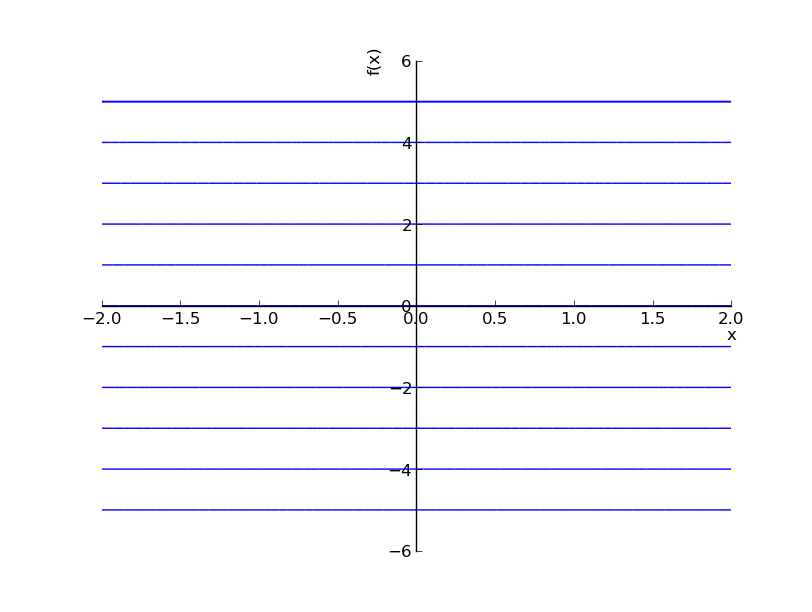
\includegraphics[scale=.3]{imagenes/sol_trivial.png}
 \end{wrapfigure}
 Hay muchas simetrías. Las traslaciones en cualquier dirección $(x,y)\mapsto (x+\alpha ,y+\beta)$ ($\alpha,\beta\in\rr$). Cambios de escala en ambos ejes  $(x,y)\mapsto (e^{\epsilon}x,y)$, $(x,y)\mapsto (x,e^{\epsilon}y)$. Reflexiones respecto ambos ejes  $(x,y)\mapsto (-x,y)$, $(x,y)\mapsto (x,-y)$.  Observar que el gráfico de las soluciones posee las mismas simetrías, pues en general \emph{las simetrías de una ecuación llevan soluciones en soluciones}.

 De todas las simetrías encontradas $\Gamma_{\epsilon}(x,y)=(e^{\epsilon}x,y)$, $\Gamma_{\epsilon}(x,y)=(x+\epsilon,y)$ y  $\Gamma_{\epsilon}(x,y)=(x+\epsilon,y)$ se llaman \emph{triviales} pues llevan una curva solución en si misma.  Cualquier cambio de la forma $\hat{x}=\hat{x}(x,y)\quad \hat{y}=y$ es trivial.  \fbox{\begin{minipage}{\textwidth}\emph{Estamos interesados en hallar grupos de Lie uniparamétricos de simetrías no triviales.}
    \end{minipage}
  }


 Las reflexiones $\Gamma(x,y)=(-x,y)$  no pertenecen a tal tipo de  grupo. Para demostrar esto supongamos que  $\Gamma$ es alguna instancia de un tal grupo $\Gamma{\epsilon}$, supongamos por ejemplo que $\Gamma=\Gamma{\epsilon_0}$.  Consideramos el jacobiano de la transformación:

\[J(\epsilon):=\det\begin{pmatrix} \frac{\partial\hat{x}}{\partial x}&  \frac{\partial\hat{x}}{\partial y}\\
 \frac{\partial\hat{y}}{\partial x} &  \frac{\partial\hat{y}}{\partial y}\\
\end{pmatrix}
\]
 Tenemos que $J(0)=1$ y $J(\epsilon_0)=-1$. Y $J(\epsilon)$ es continua respecto a $\epsilon$. Por ende existiría $\epsilon'$ con $J(\epsilon')=0$. Esto implica que la matriz jacobiana $D\Gamma$ es singular y esto contradice que $\Gamma:\rr^2\to \rr^2$ es difeomorfismo ($D\Gamma D\Gamma^{-1}=I$).



 $\Gamma$  genera un grupo discreto, ya que $\Gamma^2=\Gamma\circ \Gamma=I$. Luego $\Gamma$ genera el grupo $G=\{I,\Gamma\}$ que es isomorfo a $\mathbb{Z}_2$. En este caso diremos que    $\{I,\Gamma\}$ es un \emph{grupo discreto} de simetrías.




 \begin{ejemplo} Hallar simetrías de
\[\frac{dy}{dx}=f(x).\]
\end{ejemplo}
De acuerdo con \eqref{eq:subsder} se debe cumplir que
 \[\frac{\frac{\partial\hat{y}}{\partial x}+\frac{\partial\hat{y}}{\partial y}f(x)}{\frac{\partial\hat{x}}{\partial x}+\frac{\partial\hat{x}}{\partial y}f(x)}=f(\hat{x})\]
La forma de la ecuación sugiere el  \href{http://es.wikipedia.org/wiki/Ansatz}{ansatz}
   \[\boxed{\hat{x}=x},\quad \frac{\partial\hat{y}}{\partial x}=\frac{\partial\hat{x}}{\partial y}=0,\quad
   \frac{\partial\hat{y}}{\partial y}=\frac{\partial\hat{x}}{\partial x}. \]
 Luego 
\[\frac{\partial\hat{y}}{\partial y}=1\Rightarrow \boxed{\hat{y}=y+\epsilon} \]
con $\epsilon$ constante arbitraria. Hallamos que
\[\Gamma_{\epsilon}(x,y)=(x,y+\epsilon)\]
es un grupo de Lie uniparamétrico de simetrías. De manera similar
\[\Gamma_{\epsilon}(x,y)=(x+\epsilon,y)\]
es un grupo uniparamétrico de simetrías para 
\[\frac{dy}{dx}=f(y).\]
Geométricamente en el primer caso todas las soluciones se obtienen trasladando una cualquiera verticalmente y en el segundo caso horizontalmente.



\begin{tabular}{cc}
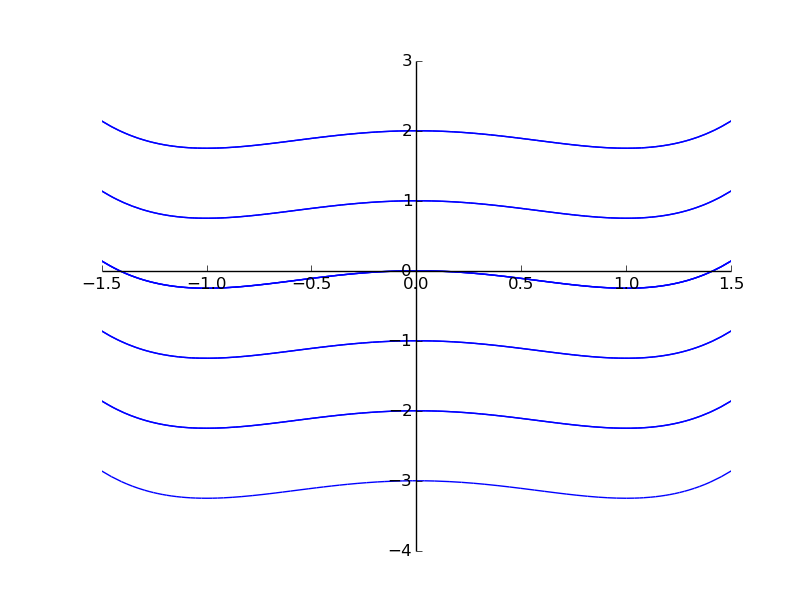
\includegraphics[scale=.3]{imagenes/sol_paralelas.png} &\hspace{-1.5cm}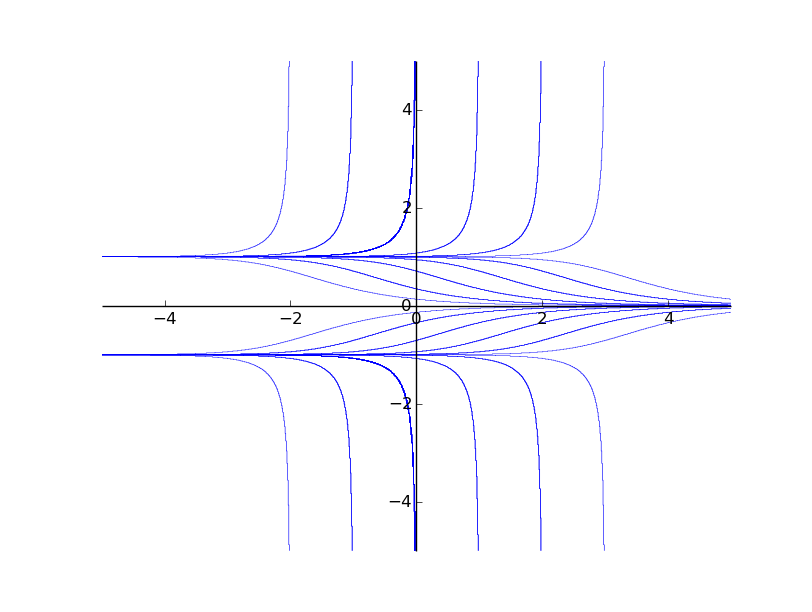
\includegraphics[scale=.3]{imagenes/sol_paralelas2.png} \\
Soluciones de $y'=x^3-x$ &\hspace{-1.5cm}Soluciones de $y'=y^3-y$
\end{tabular}





\begin{ejemplo}
 Demostrar que las rotaciones alrededor del origen es un grupo de Lie uniparamétrico de simetrías de
 \[\frac{dy}{dx}=\frac{y^3+x^2y-x-y}{x^3+xy^2-x+y}.\]
\end{ejemplo}
Sea $\Gamma_{\epsilon}$ la transformación que rota un ángulo $\epsilon$ alrededor del origen. Es un ejercicio demostrar que  $\{\Gamma_{\epsilon}|\epsilon\in\rr\}$ es un grupo uniparamétrico de simetrías. Se tiene la representación matricial
\[
\Gamma_{\epsilon}(x,y)= \begin{pmatrix} \hat{x}\\ \hat{y}
\end{pmatrix}=\begin{pmatrix} \cos(\epsilon) & -\sen(\epsilon)
\\ \sen(\epsilon) & \cos(\epsilon)
\end{pmatrix} \begin{pmatrix} x\\ y
\end{pmatrix}
\]

\[
\Gamma^{-1}_{\epsilon}(\hat{x},\hat{y})= \begin{pmatrix} x\\ y
\end{pmatrix}=\begin{pmatrix} \cos(\epsilon) & \sen(\epsilon)
\\ -sen(\epsilon) & \cos(\epsilon)
\end{pmatrix} \begin{pmatrix} \hat{x}\\ \hat{y}
\end{pmatrix}
\]


Para el cálculo recurrimos a \texttt{SymPy} (usamos \texttt{x\_n} en lugar de $\hat{x}$)
\begin{lstlisting}
from sympy import *
x,theta=symbols('x,theta')
y=Function('y')(x)
x_n=cos(theta)*x-sin(theta)*y
y_n=sin(theta)*x+cos(theta)*y
Expr2=y_n.diff(x)/x_n.diff(x)
Expr3=Expr2.subs(y.diff(),\
(y**3+x**2*y-x-y)/(x**3+x*y**2-x+y))
x_n,y_n=symbols('x_n,y_n')
Expr4=Expr3.subs([(y, -sin(theta)*x_n+cos(theta)*y_n),\
(x,cos(theta)*x_n+sin(theta)*y_n)])
Expr5=simplify(Expr4)
\end{lstlisting}



\begin{wrapfigure}[15]{r}{5.5cm}
 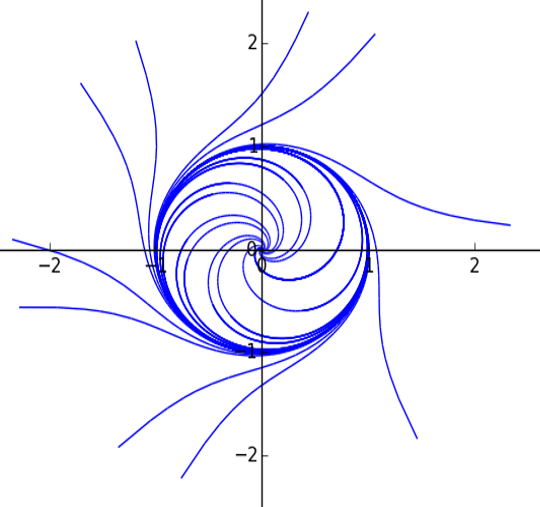
\includegraphics[scale=.4]{imagenes/sol_rotadas.png}
\end{wrapfigure}
La ecuación resultante es \emph{la misma}
\[\frac{dy_n}{dx_n}=\frac{x_{n}^{2} y_{n} - x_{n} + y_{n}^{3} - y_{n}}{x_{n}^{3} + x_{n} y_{n}^{2}
    - x_{n} + y_{n}}.\]
A la misma conclusión arribábamos si recordabamos que en en coordenadas polares la ecuación se escribe
\[\frac{dr}{d\theta}=r-r^3,\]
y que esta ecuación tiene las simetrías $\Gamma_{\epsilon}:(r,\theta)\mapsto (r,\theta+\epsilon)$. Si rotamos un ángulo fijo el gráfico de una solución obtenemos el gráfico de otra solución.










{Simetrías resuelven ecuaciones}\label{pag:sim_tras}
\textbf{Ejemplo:} Supongamos que $y'=f(x,y)$ tiene  el grupo de Lie uniparamétrico de simetrías
\boxedeq{(\hat{x},\hat{y})=\Gamma_{\epsilon}(x,y)=(x,y+\epsilon)}{eq:tras_lie}
Usando la condición de simetrías \eqref{eq:cond_sim} tenemos
\[f(x,y)=f(\hat{x},\hat{y})=f(x,y+\epsilon).\]
Luego
\[\frac{\partial f(x,y)}{\partial y}=\lim_{\epsilon\to 0}\frac{f(x,y+\epsilon)-f(x,y)}{\epsilon}=0\]
Asi $f$ es independiente de $y$: $f(x,y)=f(x)$ y la ecuación
\[y'=f(x),\]
se resuelve simplemente integrando.



\section{Órbitas, tangentes y curvas invariantes}


\begin{definicion}[Órbitas] Dado un grupo uniparamétrico de simetrías $G=\{\Gamma_{\epsilon}|\epsilon\in\rr\}$, y $(x_0,y_0)\in\rr^2$ llamamos \emph{órbita $(x_0,y_0)$ bajo la acción de  $G$} (simplemente órbita si es claro quien es $G$) a la curva
\[\{\Gamma_{\epsilon}(x_0,y_0)|\epsilon\in\rr\} \]
\end{definicion}

\begin{wrapfigure}[15]{r}{5.5cm}
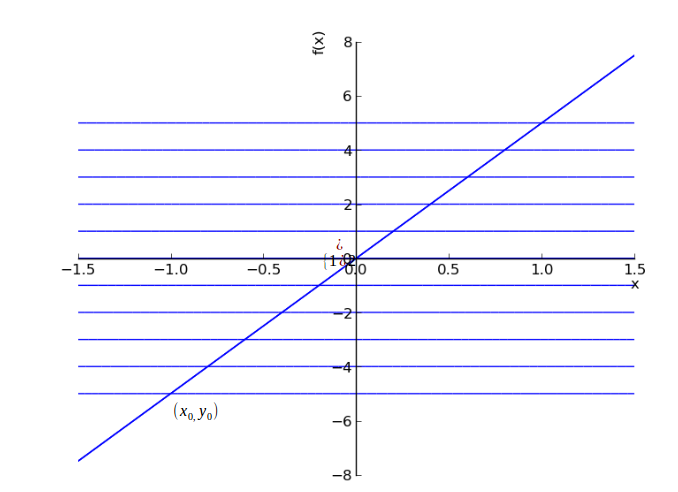
\includegraphics[scale=.3]{imagenes/sol_trivialB.png}
\end{wrapfigure}
Si $G$ es un grupo de simetrías no trivial, entonces es de esperar que la órbita de  $(x_0,y_0)$ cruce transversalmente las curvas solución. La órbita se usará como una nueva coordenada.
 La órbita atraves de $(x,y)$ es el conjunto de puntos de coordenadas
\begin{equation}\label{eq:orb} (\hat{x}(x,y,\epsilon),\hat{y}(x,y,\epsilon))=\Gamma_{\epsilon}(x,y),
\end{equation}
donde
\[(\hat{x}(x,y,0),\hat{y}(x,y,0))=(x,y).\]
Las ecuaciones \eqref{eq:orb} son ecuaciones parámetricas (parámetro $\epsilon$) de una  curva en el plano.

\begin{definicion}[Puntos invariantes]
Un punto $(x,y)$ se llama invariante si su órbita se reduce a $\{(x,y)\}$, vale decir
\[(x,y)=\Gamma_{\epsilon}(x,y),\quad\forall \epsilon>0\]
\end{definicion}






\begin{ejemplo} La órbita de $(x,y)$ bajo la acción del grupo  de Lie uniparamétrico
\[
\Gamma_{\epsilon}(x,y)= \begin{pmatrix} \hat{x}\\ \hat{y}
\end{pmatrix}=\begin{pmatrix} \cos(\epsilon) & -\sen(\epsilon)
\\ \sen(\epsilon) & \cos(\epsilon)
\end{pmatrix} \begin{pmatrix} x\\ y
\end{pmatrix}
\]
Son circunsferencias con centro en el origen. El punto $(0,0)$ es invariante.

\end{ejemplo}


\begin{definicion}[Campo vectorial de tangentes]
 Dado un grupo de Lie uniparamétrico $(\hat{x}(x,y,\epsilon),\hat{y}(x,y,\epsilon))=\Gamma_{\epsilon}(x,y)$  definimos el campo vectorial
\[(\xi(\hat{x},\hat{y}),\eta(\hat{x}, \hat{y}))=\left(\left.\frac{d\hat{x}}{d\epsilon}\right|_{\epsilon=0}, \left.\frac{d\hat{y}}{d\epsilon}\right|_{\epsilon=0}   \right).\]
 $\xi$ y $\eta$ se llaman \emph{símbolos infinitesimales}.
\end{definicion}

 Como $\hat{x},\hat{y}$ eran analíticas respecto a $\epsilon$ :
\[
\begin{array}{cc}
\hat{x}&=x+\epsilon\xi(x,y)+O(\epsilon^2)\\
\hat{y}&=y+\epsilon\eta(x,y)+O(\epsilon^2)\\
\end{array}
\]
 En un punto invariante \fbox{$\xi(x,y)=\eta(x,y)=0$}.



[fragile]{Campo vectorial de tangentes}
\begin{lstlisting}
x,y,epsilon = var('x,y,epsilon')
x_n=cos(epsilon)*x-sin(epsilon)*y
y_n=sin(epsilon)*x+cos(epsilon)*y
xi=x_n.diff(epsilon)(epsilon=0)
eta=y_n.diff(epsilon)(epsilon=0)
p=plot([])
for x_abs in srange(0,1,.2):
    p+=parametric_plot([x_n(x=x_abs,y=0),\
y_n(x=x_abs,y=0)], (epsilon,0,2*pi))
p+= plot_vector_field((xi,eta),(x,-1,1),\
(y,-1,1))
\end{lstlisting}




[fragile]{Campo vectorial de tangentes}
plot[scale=.5]{p}




{Curvas invariantes}
{Definición}
Una curva plana $C$ se dice invariante por un grupo uniparamétrico de simetrías de Lie si y sólo si la tangente a  $C$ en cada punto $(x,y)$ es paralela a $(\xi(x,y),\eta(x,y))$. Si $C$ es el gráfico de una función $x\mapsto y(x)$, como $(1,y'(x))$ es un vector tangente a la gráfica, la condición que $C$ es invariante se escribe
\boxedeq{Q(x,y,y')\overset{\hbox{\small def}}{=}\eta(x,y)-y'\xi(x,y)\equiv 0}{eq:inv}
Esta se llama \emph{ecuación característica}.






{Curvas invariantes}
 {Soluciones invariantes}
Si $\Gamma_{\epsilon}$ es un grupo de Lie de simetrías de $y'=f(x,y)$ entonces una solución $y(x)$ es una curva invariantes si y sólo si
\boxedeq{\overline{Q}(x,y)=\eta(x,y)-f(x,y)\xi(x,y)\equiv 0}{eq:sol_inv}

Se llaman \emph{ecuación característica reducida}.


 \emph{Nos conviene tener soluciones no invariantes}




{Ejemplos}
\textbf{Ejemplo:} La EDO
\[y'=y\]
Tiene simetrías de escala
\[(\hat{x},\hat{y})=\Gamma_{\epsilon}(x,y)=(x,e^{\epsilon}y).\]
Luego 
\[(\xi,\eta)=\left(\left.\frac{d\hat{x}}{d\epsilon}\right|_{\epsilon=0}, \left.\frac{d\hat{y}}{d\epsilon}\right|_{\epsilon=0}   \right)=(0,y)\]
Cualquier punto en el conjunto $\{(x,0)|x\in\rr\}$  es invariante. La ecuación característica reducida es.
\[\overline{Q}(x,y)=0\Rightarrow y=0\]
Esta formada enteramente por puntos invariantes.




{Ejemplos}

\textbf{Ejercicio:} demostrar que la siguiente expresión es un grupo de Lie uniparamétrico de simetrías
\[(\hat{x},\hat{y})=\Gamma_{\epsilon}(x,y)=(e^{\epsilon}x,e^{(e^{\epsilon}-1)x}y).\]
Para este grupo tenemos
\[(\xi,\eta)=(x,xy)\]
Todo punto en $x=0$ es invariante. La ecuación característica reducida es
\[\overline{Q}(x,y)=0\Rightarrow xy-xy=0\]
De modo que estas simetrías actuan trivialmente sobre las soluciones. Llevan una solución en si misma. Chequeemos esta afirmación de manera directa. 





{Ejemplos}
Buscamos el cambio de variables inverso
\[
\left.
\begin{array}{ll} 
  \hat{x}&= e^{\epsilon}x\\
  \hat{y}&=e^{(e^{\epsilon}-1)x}y\\
\end{array}
\right\} 
\Rightarrow  
    \left.
\begin{array}{ll} 
  x&= e^{-\epsilon}\hat{x}\\
  y&=e^{(e^{-\epsilon}-1)\hat{x}}\hat{y}\\
\end{array}
\right\} 
\]    

Las soluciones son $y=ke^x$, sustituímos en esta expresión, luego de unas operaciones, llegamos a $\hat{y}=ke^{\hat{x}}$.




{Ejemplos}

\textbf{Ejemplo.} La ecuación de Riccati
\[y'=xy^2-\frac{2y}{x}-\frac{1}{x^3},\quad x\neq 0\] 
 Tiene el grupo de Lie de simetrías
\[(\hat{x},\hat{y})=\Gamma_{\epsilon}(x,y)=(e^{\epsilon}x,e^{-2\epsilon}y).\]
Tenemos
\[(\xi,\eta)=(x,-2y).\]
La característica reducida
\[\overline{Q}(x,y)=\frac{1}{x^2}-x^2y^2=0.\]
Tenemos dos soluciones invariantes
\[y=\pm\frac{1}{x^2}.\] 




{Infinitesimales$\to$Simetrías}

 La mayoría de los métodos de simetría usan  $(\xi,\eta)$ en lugar de las simetrías en si mismas.
Por otra parte  $(\xi(\hat{x},\hat{y}),\eta(\hat{x},\hat{y}))$ determinan las simetrías a traves de las ecuaciones

\boxedeq{
\left\{
\begin{array}{ll}
\frac{d\hat{x}}{d\epsilon}&=\xi(\hat{x},\hat{y})\\
\frac{d\hat{y}}{d\epsilon}&=\eta(\hat{x},\hat{y})\\
\hat{x}(x,y,0)&=x\\
\hat{y}(x,y,0)&=y\\
\end{array}
\right.
}{eq:ecua_infinitesimales}

\textbf{Justificación de las ecuaciones}. Si ponemos $(\hat{x},\hat{y})=\Gamma_{\epsilon}(x,y)$, de la propiedad de grupo ($ \Gamma_{\Delta\epsilon} \circ  \Gamma_{\epsilon}= \Gamma_{\epsilon+\Delta\epsilon}$), deducimos 
\[\hat{x}(\Gamma_{\epsilon}(x,y),\Delta\epsilon)=\hat{x}(x,y,\epsilon+\Delta\epsilon).\]




{Infinitesimales$\to$Simetrías}
Luego

\[
\begin{split}
\frac{d\hat{x}}{d\epsilon}&=\lim_{\Delta\epsilon\to 0}\frac{\hat{x}(x,y,\epsilon+\Delta\epsilon)-\hat{x}(x,y,\epsilon)  }{\Delta\epsilon}\\
&=\lim_{\Delta\epsilon\to 0}\frac{\hat{x}(\Gamma_{\epsilon}(x,y),\Delta\epsilon)  -\hat{x}(x,y,\epsilon)  }{\Delta\epsilon}\\
&=\lim_{\Delta\epsilon\to 0}\frac{\hat{x}(\hat{x}(x,y,\epsilon),\hat{y}(x,y,\epsilon),\Delta\epsilon)  -\hat{x}(\hat{x}(x,y,\epsilon),\hat{y}(x,y,\epsilon),0)  }{\Delta\epsilon}\\
&=\left.\frac{d\hat{x}}{d\epsilon}\right|_{\epsilon=0}=\xi(\hat{x},\hat{y})
\end{split}
\]


{Infinitesimales$\to$Simetrías}

El \emph{sistema de ecuaciones} \eqref{eq:ecua_infinitesimales}    pueden ser dificiles de resolver. Pero en algunos casos sencillos puede ser fácil.

 \textbf{Ejemplo:} Encontrar el grupo de simetrías para los infinitesimales $\xi(x,y),\eta(x,y))=(x^2,xy)$.


\[ \frac{d\hat{x}}{d\epsilon}=\xi(\hat{x},\hat{y})=\hat{x}^2\text{ y }\hat{x}(x,y,0)=x
\Rightarrow \hat{x}=\frac{x}{1-\epsilon x}\]
y

\[ \frac{d\hat{y}}{d\epsilon}=\eta(\hat{x},\hat{y})=\hat{x}\hat{y}\text{ y }\hat{y}(x,y,0)=y
\Rightarrow \hat{y}=\frac{y}{1-\epsilon x}\]






\section{Coordenadas canónicas}

{Coordenadas canónicas}
 {Definición}   Diremos que las coordenadas $(r,s)$ son canónicas respecto a el grupo de Lie de simetrías $\Gamma{\epsilon}$  si en las coordenadas $(r,s)$ la acción de grupo es la traslación

\boxedeq{(\hat{r},\hat{s})\overset{\hbox{def}}{=} (r(\hat{x},\hat{y}),s(\hat{x},\hat{y}))=(r(x,y),s(x,y)+\epsilon).}{eq:coorcan}

 \textbf{Ejemplo:} Las coordenadas polares son canónicas respecto al grupo de Lie de rotaciones. Las rotaciones en coordenadas cartesianas y polares se escriben
\[
 \begin{pmatrix} \hat{x}\\ \hat{y}
\end{pmatrix}=\begin{pmatrix} \cos(\epsilon) & -\sen(\epsilon)
\\ \sen(\epsilon) & \cos(\epsilon)
\end{pmatrix} \begin{pmatrix} x\\ y
\end{pmatrix},\quad \begin{array}{ll} \hat{r}&=r\\ \hat{\theta}&=\theta+\epsilon\\ 
\end{array}
\]


{Coordenadas canónicas}
 Derivando las ecuaciones \eqref{eq:coorcan} respecto a $\epsilon$ obtenemos
\boxedeq{
\begin{array}{ll}
\xi(x,y)\frac{\partial r}{\partial x}+\eta(x,y)\frac{\partial r}{\partial y}&=0\\
\xi(x,y)\frac{\partial s}{\partial x}+\eta(x,y)\frac{\partial s}{\partial y}&=1
\end{array}
}{eq:coor_can_dif}
 Los cambios de coordenadas deben ser invertibles, de modo que pediremos la condición de no degeneración
\boxedeq{\frac{\partial r}{\partial x}\frac{\partial s}{\partial y}-\frac{\partial r}{\partial y}\frac{\partial s}{\partial x}\neq 0}{eq:no_deg}

 {Extensión definición}
Cualquier par de coordenadas que satisfacen \eqref{eq:coor_can_dif} y \eqref{eq:no_deg} se llaman canónicas.







{Coordenadas canónicas}

 {Observaciones}
\begin{enumerate}
\item El vector tangente en cualquier punto no invariante es paralelo a la curva $r=\hbox{cte}$ que pasa por ese punto. Luego esa curva es una órbita. Las órbitas son invariantes, así  $r$ se llama la \emph{coordenada invariante}. Las curvas $s=\hbox{cte}$ son transversales a las órbitas.
\item Las coordenadas canónicas no estan definidas en un punto $(x,y)$ invariante pues en esos puntos $\xi(x,y)=\eta(x,y)=0$.

\item Las coordenadas canónicas estan definidas en un entorno de cualquier   punto no invariante.

\item Las coordenadas canónicas no son únicas. De hecho si $(r,s)$ son canónicas $(\tilde{r},\tilde{s})=(F(r),G(r)+s)$ lo son para cualquier $F$ y $G$ con $F'(r)\neq 0$ para la no degeneración.

\end{enumerate}







{Coordenadas canónicas}
 {Generador Infinitesimal}
Al operador diferencial
\boxedeq{X=\xi(x,y)\frac{\partial }{\partial x}+\eta(x,y)\frac{\partial }{\partial y}}{eq:generador_infinitesimal}
se lo suele denominar \emph{Generador Infinitesimal}. La acción del operador sobre una función $f$ diferenciable es tomar la derivada direccional en la dirección del campo $(\xi,\eta)$. 


Las ecuaciones \eqref{eq:coor_can_dif} se escriben de manera compacta
\boxedeq{
\begin{array}{ll}
Xr&=0\\
Xs&=1
\end{array}
}{eq:coor_can_difb}
La primera expresa que $r$ no cambia en la dirección del campo.








{Encontrando coordenadas canónicas}

 {Integrales primeras}
Una integral primera de la EDO $y'=f(x,y)$ es una función $\phi(x,y)$ que es constante a lo largo de una curva solución de la EDO. 


 {Teorema} Si $(r,s)$ son coordenadas canónicas de una grupo de Lie de simetrías entonces $r$ es una integral primera de la ecuación
\begin{equation}\label{eq:int_pri} \frac{dy}{dx}=\frac{\eta(x,y)}{\xi(x,y)}.
\end{equation}






{Encontrando coordenadas canónicas}

\textbf{Dem.} Supongamos $y(x)$ solución de la EDO, es suficiente demostrar que $\frac{d}{dx}r(x,y(x))=0$. En efecto
\[
\begin{array}{lll}
 \frac{d}{dx}r(x,y(x)) &=\frac{\partial r}{\partial x}+\frac{\partial s}{\partial y}y' &\text{(regla cadena)}\\
&=\frac{\partial r}{\partial x}+\frac{\partial s}{\partial y}\frac{\eta(x,y)}{\xi(x,y)}& \text{(Ec. \eqref{eq:int_pri})}\\
&=0 & \text{(Ec. \eqref{eq:coor_can_dif})}\\
\end{array}
\]





{Encontrando coordenadas canónicas}
Hallar una integral primera implica resolver la ecuación.
\textbf{Ejemplo} Ya conocemos las coordenadas canónicas de las rotaciones, 
\[
 \begin{pmatrix} \hat{x}\\ \hat{y}
\end{pmatrix}=\begin{pmatrix} \cos(\epsilon) & -\sen(\epsilon)
\\ \sen(\epsilon) & \cos(\epsilon)
\end{pmatrix} \begin{pmatrix} x\\ y
\end{pmatrix}\Rightarrow  \begin{pmatrix} \xi\\ \eta
\end{pmatrix}= \begin{pmatrix} -y\\ x
\end{pmatrix}
\]
hallemosla por el método propuesto. Hay que resolver 
\[\frac{dy}{dx}=-\frac{x}{y}\Rightarrow ydy=-xdx\Rightarrow y^2+x^2=C\]
Luego $r=\sqrt{x^2+y^2}$ es una integral primera. 






{Encontrando coordenadas canónicas}
La coordenada $r$ es constante sobre los puntos en la gráfica de una solución de \eqref{eq:int_pri}. Sobre esos puntos $(x,y(x))$, la coordenada $s$ satisface:

\begin{equation} \label{eq:coor_can_s}
\begin{array}{lll}
\frac{ds}{dx}&=\frac{\partial s}{\partial x}+\frac{\partial s}{\partial y} y'(x) & \hbox{(Regla cadena)}\\
&=\frac{\partial s}{\partial x}+\frac{\partial s}{\partial y} \frac{\eta}{\xi} &
  \eqref{eq:int_pri}\\
&=\frac{1}{\xi} &\hbox{\eqref{eq:coor_can_dif}}.
\end{array}
\end{equation}

Ahora podemos aprovechar que ya conocemos $r$ y  expresar $y$ como función de $r,x$. Luego

{Teorema: Expresión para $s$}
\boxedeq{s=\int\frac{ds}{dx}dx=\int\frac{dx}{\xi(x,y(r,x))}.}{eq:expr_coor_s}
 


 











{Encontrando coordenadas canónicas}
En la igualdad resultante puede ser necesario reemplazar $r$ por su expresión en las variables $x,y$.


Si ocurriese que $\xi=0$ y $\eta\neq 0$. Entonces por \eqref{eq:int_pri} $r_y=0$, de modo que $r$ es sólo función de $x$. Se puede asumir $r=x$. Además $\eta s_y=1$, entonces
\boxedeq{s=\int\frac{dy}{\eta(r,y)} .}{eq:s_xi_0}


\textbf{Ejemplo} Retornando al ejemplo de las rotaciones, donde hallamos que $r=\sqrt(x^2+y²)$, vemos que

\[s=\int\frac{dx}{-y}=-\int\frac{dx}{\sqrt{r^2-x^2}}=\arccos\left(\frac{x}{r}\right).\]
Por consiguiente  $s$ es el ángulo polar.





{Encontrando coordenadas canónicas}\label{pag_ejem_canon1}
\textbf{Ejemplo} Encontrar coordenadas canónicas para el grupo de Lie de simetrías
\[(\hat{x},\hat{y})=(e^{\epsilon}x,e^{k\epsilon}y)\quad k>0.\]
El vector tangente es
\[(\xi,\eta)=\left(\left.\frac{d\hat{x}}{d\epsilon}\right|_{\epsilon=0},\left.\frac{d\hat{y}}{d\epsilon}\right|_{\epsilon=0}\right)=(x,ky).\]
Resolvamos la ecuación  \eqref{eq:int_pri} 
\[\frac{dy}{dx}=\frac{ky}{x}\Rightarrow y=Cx^k.\]
Luego $\Phi=y/x^k$ es integral primera. Entonces podemos tomar $r=y/x^k$. 









{Encontrando coordenadas canónicas}\label{pag_ejem_canon2}
 Para $s$
\[s=\int\frac{dx}{\xi}=\frac{dx}{x}=\ln|x|.\]
Entonces $(r,s)=(yx^{-k},\ln|x|)$ son coordenadas canónicas. No estan definidas en $x=0$.
Podemos encontrar coordenadas canónicas definidas en $x=0$ del siguiente modo. Recordamos que para todas $F$ y $G$
\[(\tilde{r},\tilde{s})=(F(r),G(r)+s)=(F(x^{-k}y),G(x^{-k}y)+\ln|x|).\]
So canónicas también. Si tomamos $F(r)=1/r$ y $G(r)=\frac{1}{k}\ln|r|$, evitamos la singularidad. Luego

\[(\tilde{r},\tilde{s})=(x^ky^{-1},\frac{1}{k}\ln|y|).\]
Son canónicas, están definidas en $x=0$ pero no en $y=0$.  









{Encontrando coordenadas canónicas}\label{pag:can_ejem_p}
\textbf{Ejemplo} Encontrar coordenadas canónicas para
\[(\hat{x},\hat{y})=\left( \frac{x}{1-\epsilon x},\frac{y}{1-\epsilon x}\right).\]

\[(\xi,\eta)=\left(\left.\frac{d\hat{x}}{d\epsilon}\right|_{\epsilon=0},\left.\frac{d\hat{y}}{d\epsilon}\right|_{\epsilon=0}\right)=(x^2,xy).\]

\[\frac{dy}{dx}=\frac{\eta}{\xi}=\frac{y}{x}\Rightarrow \frac{y}{x}=\hbox{cte}.\]

Podemos tomar $r=y/x$. Para $s$
\[s=\int\frac{dx}{x^2}=-\frac{1}{x}.\]
Luego $(r,s)=(\frac{y}{x},-\frac{1}{x})$ son canónicas.



En este caso los puntos sobre $x=0$ son invariantes, no podemos definir coordenadas canónicas allí.


 




[fragile]{Encontrando coordenadas canónicas}
Lo podemos desarrollar con \texttt{SymPy}. 
\begin{lstlisting}
sage: from sympy import *
sage: x,y,epsilon=symbols('x,y,epsilon')
sage: T=Matrix([x/(1-epsilon*x),y/(1-epsilon*x)])
sage: xi=T[0].diff(epsilon).subs(epsilon,0)
sage: xi
sage: eta=T[1].diff(epsilon).subs(epsilon,0)
sage: eta/xi
sage: y=Function('y')(x)
sage: dsolve(y.diff(x)-y/x,y)


\end{lstlisting}


[fragile]{Encontrando coordenadas canónicas}
 
\begin{lstlisting}
sage: Integral(1/xi,x).doit()

\end{lstlisting}





{Infinitesimales$\to$Simetrías (Revisitado)}
Las coordenadas canónicas nos dan otra manera de encontrar simetrías a partir de los infinitesimales siguiendo el procedimiento:

\begin{enumerate}
\item Determinar las coordenadas canónicas  (sólo necesitamos conocer los infinitesimales).
\item Expresamos las relaciones $\hat{r}=r$ y $\hat{s}=s+\epsilon$ en las coordenadas $x,y$.
\end{enumerate}


\textbf{Ejemplo:} Hallar el grupo de simetrías asociado al generador infinitesimal
\[X=x^2\frac{\partial}{\partial x}+xy\frac{\partial}{\partial y}.\]


{Infinitesimales$\to$Simetrías (Revisitado)}
 Las coordenadas canónicas nos dan otra manera de encontrar simetrías a partir de los infinitesimales siguiendo el procedimiento:

\begin{enumerate}
\item En la página \ref{pag:can_ejem_p} hallamos las coordenadas canónicas asociadas a los infinitesimales $(r,s)=\left(\frac{y}{x},-\frac{1}{x}\right)$
\item Ahora
\[\begin{split}
(\hat{r},\hat{s})&=(r,s+\epsilon)\Rightarrow \frac{\hat{y}}{\hat{x}}=\frac{y}{x}\text{ , }-\frac{1}{\hat{x}}=-\frac{1}{x}+\epsilon\\
&\Rightarrow \hat{x}=\frac{x}{1-\epsilon x} \text{ , } \hat{y}=\frac{y}{1-\epsilon x}.
\end{split}
\] 
\end{enumerate}



\section[Resolviendo EDO]{Resolviendo EDO con grupos de Lie de simetrías}

{Resolviendo EDO con grupos de Lie de simetrías}

 Supongamos dado  un grupo de Lie de simetrías $(\hat{x},\hat{y})$ de la ecuación
\boxedeq{y'=f(x,y)}{eq:eq_princi}

 Supongamos  que las simetrías son no triviales. Según \eqref{eq:sol_inv} debemos tener
 \[\eta(x,y)\not\equiv f(x,y)\xi(x,y)\]
La razón de esta condición es que si fuese falsa entonces la ecuación \eqref{eq:int_pri} es la misma que la ecuación \eqref{eq:eq_princi} y el método es inútil.

Supongamos $(r,s)$ coordenadas canónicas. La ecuación en las coordenadas $(r,s)$, según \eqref{eq:subsder}, se escribirá
\boxedeq{\frac{ds}{dr}=\hat{f}(r,s):=\frac{s_x+f(x,y)s_y}{r_x+f(x,y)r_y}.}{eq:prin_en_canon}
 



{Resolviendo EDO con grupos de Lie de simetrías}
Las coordenadas canónicas se definen por \eqref{eq:coorcan} de modo que el grupo de simetrías actúe por traslación $(\hat{r},\hat{s})=(r,s+\epsilon)$.
Por los resultados de la página  \ref{pag:sim_tras}, $\hat{f}$ es independiente de $s$. Y la ecuación se reduce a
\boxedeq{\frac{ds}{dr}=\hat{f}(r)}{eq:ecu_prin_canonica}

que se resuelve integrando.


\textbf{Ejemplo:} Resolver
\[y'=xy^2-\frac{2y}{x}-\frac{1}{x^3},\quad x\neq 0,\]
sabiendo que la ecuación es invariante para el grupo de simetrías
\[(\hat{x},\hat{y})=(e^{\epsilon}x,e^{-2\epsilon}y).\]



{Resolviendo EDO con grupos de Lie de simetrías}
Por los resultados de las páginas \ref{pag_ejem_canon1} y \ref{pag_ejem_canon2}:
\[(r,s)=(x^2y,\ln|x|)\]
son canónicas.

 Según \eqref{eq:prin_en_canon} la ecuación en $(r,s)$ es:
\[\frac{dr}{ds}=\frac{\frac{1}{x}}{2xy+x^2\left(  xy^2-\frac{2y}{x}-\frac{1}{x^3}     \right)}=\frac{1}{x^4y^2-1}=\frac{1}{r^2-1}\]
Como sabíamos que debía suceder el resultado del segundo miembro ndepende sólo de $r$. Integrando
\[s=\frac12\ln\left( \frac{r-1}{r+1}  \right)+C.\]
Sustituyendo
\[\ln|x|=\frac12\ln\left( \frac{x^2y-1}{x²y+1}  \right)+C.\]






{Resolviendo EDO con grupos de Lie de simetrías}
Despejando
\boxedeq{y =-\frac{x^2 + C}{x^2(x^2 - C)}}{eq:sol_ejem}
La ecuación característica reducida \eqref{eq:sol_inv} es para la ecuación de este ejemplo:

\[0=\overline{Q}=-2y- \left(xy^2-\frac{2y}{x}-\frac{1}{x^3}  \right)x=-x^2y^2+\frac{1}{x^2}\]
Cuyas soluciones son
\[y=\pm\frac{1}{x^2}.\]
Que además son solución de la ecuación diferencial. La curva $y=-1/x^2$ se obtiene de \eqref{eq:sol_ejem} con $C=0$. La  curva $y=-1/x^2$




{Resolviendo EDO con grupos de Lie de simetrías}

\begin{tabular}{m{0.3\linewidth} >{\centering\arraybackslash}m{0.7\linewidth} }
Las curvas azules y naranjas se corresponden con las gráficas de \eqref{eq:sol_ejem} con $c>0$ y $c<0$ respectivamente. La verde es la de $y=1/x^2$ y la roja de $y=-1/x^2$.
&
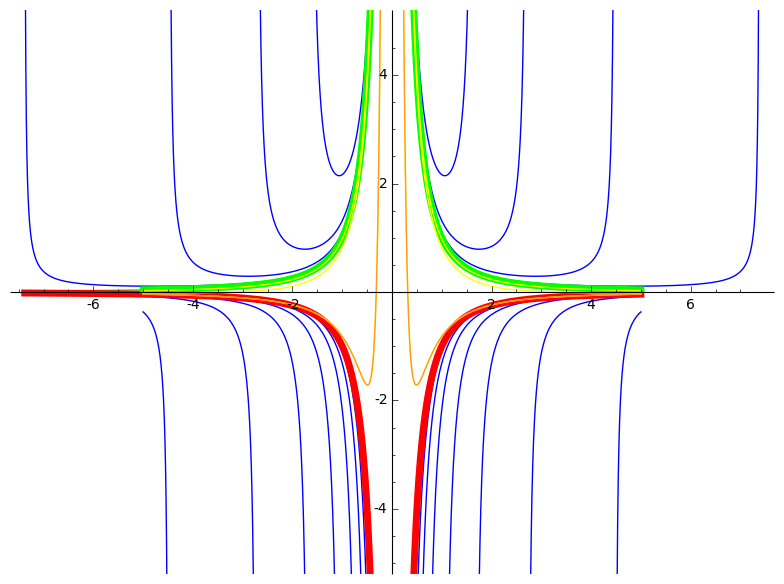
\includegraphics[scale=.4]{imagenes/SolGrup.png}
\end{tabular}




{Resolviendo EDO con grupos de Lie de simetrías}



\textbf{Ejemplo:} Resolver
\[y'=\frac{y+1}{x}+\frac{y^2}{x^3},\quad x\neq 0,\]
sabiendo que la ecuación es invariante para el grupo de simetrías
\[(\hat{x},\hat{y})=(\frac{x}{1-\epsilon x},\frac{y}{1-\epsilon x}   ).\]
Ya hemos computado las coordenadas canónicas en página \ref{pag:can_ejem_p}:
\[(r,s)=\left(\frac{y}{x},\frac{1}{x}\right).\]
Por \eqref{eq:prin_en_canon} la ecuación se escribe
\[\frac{dr}{ds}=\frac{-\frac{1}{x^2} }{-\frac{y}{x^2}+\frac{1}{x}\left(
\frac{y+1}{x}+\frac{y^2}{x^3}\right)}=\frac{1}{1+r^2}\]





{Resolviendo EDO con grupos de Lie de simetrías}
Cuya solución es 
\[s=\arctan(r)+C\Rightarrow y=-x\tan\left(\frac{1}{x}+C\right).\]



{Ecuaciones homogéneas}
\textbf{Ejemplo:} Resolver la ecuación 
\boxedeq{y'=F\left(\frac{y}{x}\right).}{eq:homogenea}
Aquí tenemos el Grupo de Lie de simetrías de cambio de escalas
\[(\hat{x},\hat{y})=(e^{\epsilon}x,e^{\epsilon}y).\] 

Por los resultados de páginas \ref{pag_ejem_canon1} y \ref{pag_ejem_canon2}, $(r,s)=(y/x,\ln|x|)$ son canónicas y la ecuación se escribe
\[\frac{ds}{dr}=\frac{\frac{1}{x}}{-\frac{y}{x^2}+\frac{F\left(\frac{y}{x}\right)}{x}}=\frac{1}{F(r)-r}.\]
La solución general es 
\[\ln|x|=\int^{y/x}\frac{dr}{F(r)-r}+c.\]




{Método de Lie y \texttt{SymPy}}
\text{SymPy} Incorpora distintas estrategías para resolver ecuaciones por el método de Lie. Hay mucho por indagar al respecto, pero sólo vamos a mencionar una función para calcular los infinitesimales $(\xi,\eta)$.  Aprovechamos para mostrar como luce una consola de \texttt{ipython}, otra manera de usar \texttt{Python} y \texttt{SymPy}.

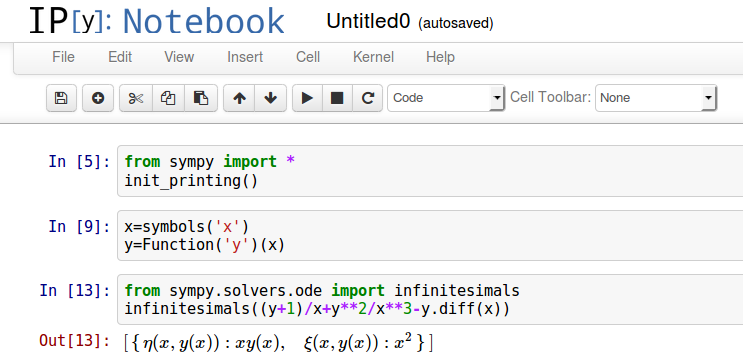
\includegraphics[scale=.45]{imagenes/ipython.png}





\end{document}

